\documentclass[UTF8,fontset=fandol,11pt]{ctexart}
\usepackage[a4paper,margin=24mm,headheight=15pt]{geometry}
\usepackage{amsmath,amssymb,amsthm,mathtools,bm}
\usepackage{enumitem,booktabs,longtable,array,pdfpages,fancyhdr,xcolor}
\usepackage[colorlinks=true,linkcolor=blue!45!black,urlcolor=blue!45!black]{hyperref}
\allowdisplaybreaks[2]
\setlength{\parindent}{2em}
\setlength{\parskip}{3pt}
\setlength{\emergencystretch}{3em}
\setlist{nosep,topsep=3pt}
\pagestyle{fancy}\fancyhf{}\fancyhead[L]{\small 分析学讲义习题解答}\fancyhead[R]{\small 第38--57讲}\fancyfoot[C]{\thepage}
\newcommand{\R}{\mathbb R}\newcommand{\C}{\mathbb C}\newcommand{\N}{\mathbb N}\newcommand{\Z}{\mathbb Z}\newcommand{\Q}{\mathbb Q}\newcommand{\T}{\mathbb T}
\newcommand{\dd}{\,\mathrm d}\newcommand{\eps}{\varepsilon}\newcommand{\ind}{\mathbf1}
\newcommand{\norm}[1]{\left\lVert#1\right\rVert}\newcommand{\abs}[1]{\left|#1\right|}\newcommand{\ip}[2]{\left\langle#1,#2\right\rangle}
\DeclareMathOperator{\supp}{supp}\DeclareMathOperator{\rank}{rank}\DeclareMathOperator{\Span}{Span}\DeclareMathOperator{\diag}{diag}\DeclareMathOperator{\Res}{Res}\DeclareMathOperator{\Ext}{Ext}
\newcommand{\problem}[2]{\subsection*{#1}\addcontentsline{toc}{subsection}{#1}\noindent\textbf{题干。}#2\par\smallskip\noindent\textbf{解答。}}
\newcommand{\fix}[1]{\par\noindent\textcolor{red!55!black}{\textbf{原文核对与修正。}#1}\par}
\newcommand{\skipnote}[1]{\par\noindent\textbf{依约不解的计算题。}#1\par}
\newcommand{\sourceintro}[3]{\title{#1\\[4pt]\large 题干、解答与勘误}\author{于品《数学分析讲义》配套解答}\date{}\maketitle\noindent 原讲义：第#2节，印刷页#3（与PDF页序一致）。题干按数学内容重排；完整原题页附于文末，含未解的传统计算题，供逐字核对。原文中的作业提交说明及引文不作为本项目的工作指令。\par 本文中的“正函数”均按非负函数理解。复内积约定对第一个变量线性。}
\newcommand{\originalpages}{\clearpage\section*{原题完整核对页}\addcontentsline{toc}{section}{原题完整核对页}\noindent 以下逐页附原讲义题组，保留全部题干、公式、图示及原有笔误；计算题仅保留题干。\clearpage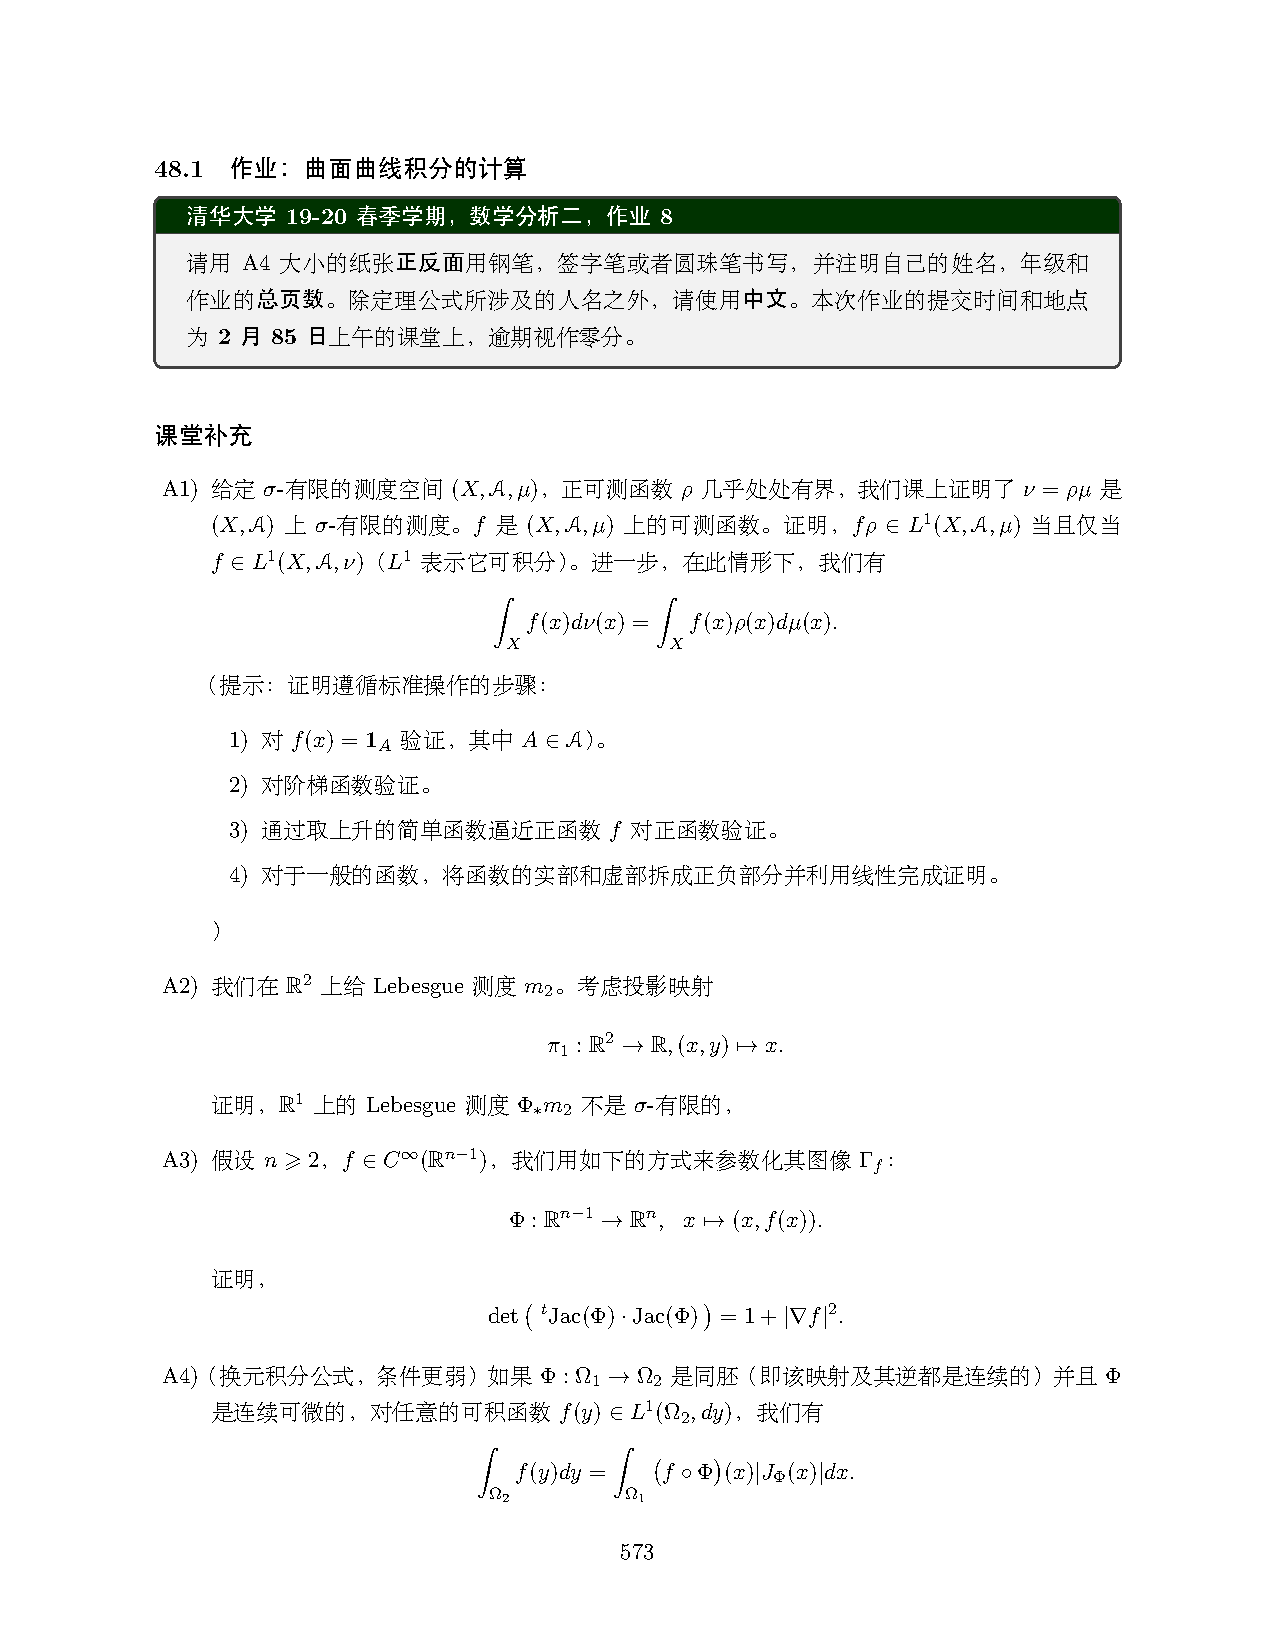
\includepdf[pages=-,pagecommand={\thispagestyle{empty}},scale=.94]{original.pdf}}

\begin{document}
\sourceintro{48.1 作业：换元、子流形测度与壳层定理}{48.1}{573--577}
\section*{所用知识}
第43--48讲：Fubini、换元、子流形体积、单位分解及等维$C^1$映射临界值零测引理。不调用一般面积公式或一般余面积定理，而在A6中证明所需的特殊情形。
\problem{A1}{给定$\sigma$-有限测度空间，$\rho\ge0$可测且几乎处处有界，$\nu=\rho\mu$。证明$f\rho\in L^1(\mu)$当且仅当$f\in L^1(\nu)$，且$\int f\dd\nu=\int f\rho\dd\mu$。}
对$f=\ind_A$，此式正是$\nu$的定义；对非负简单函数由线性成立；取非负简单函数递增逼近任意非负$f$，两边用单调收敛。应用于$|f|$得到可积性等价，然后对复函数的实虚部正负部分应用该等式。实际上只需$\rho$几乎处处有限即可保证$\nu$仍$\sigma$-有限，等式本身连此条件也无需。
\problem{A2}{令$\pi_1:\R^2\to\R$为第一投影。证明像测度$\pi_{1*}m_2$不是$\sigma$-有限。}
\fix{原文将像测度称为“$\R$上的Lebesgue测度”并把$\pi_1$误写为$\Phi$。它并不是一维Lebesgue测度。}
对Borel集$A$，$m_2(A\times\R)$在$m_1(A)=0$时为零，在$m_1(A)>0$时为无穷，因为截断$A\times[-N,N]$的测度为$2Nm_1(A)$。所以像测度有限的集合必须是一维零测集，它们的可数并不能覆盖$\R$。
\problem{A3}{对光滑$f:\R^{n-1}\to\R$和图像参数化$\Phi(x)=(x,f(x))$，证明$\det(D\Phi^TD\Phi)=1+|\nabla f|^2$。}
Gram矩阵为$I+vv^T$，$v=\nabla f$。若$v\ne0$，它在$v$方向的特征值为$1+|v|^2$，在其正交补上为$1$；$v=0$时矩阵为单位阵。取特征值乘积。
\problem{A4}{若$\Phi:\Omega_1\to\Omega_2$为$C^1$同胚，证明对任意$f\in L^1(\Omega_2)$有$\int_{\Omega_2}f=\int_{\Omega_1}f(\Phi(x))|\det D\Phi(x)|\dd x$。}
令$C=\{\det D\Phi=0\}$，第48讲的等维Sard型引理给出$m(\Phi(C))=0$。在开集$\Omega_1\setminus C$上，反函数定理使$\Phi$为局部$C^1$微分同胚。取可数个这样的坐标邻域并作Borel不交化，在每块上应用第45讲换元公式后求和；$\Phi$单射使像块也不交。源端临界集的被积函数为零，像端临界值集也零测，故加回两者得到结论。先对非负$f$作此论证，再对$|f|$及复函数推广，也验证右端绝对可积。
\problem{A5}{对超曲面$M\subset\R^n$及投影$\pi:M\to\R^{n-1}$，证明$\pi(\operatorname{Sing}\pi)$零测，且它恰由与$M$相切的竖直直线$L_{x'}=\{(x',t)\}$的参数$x'$组成。}
在可数个子流形坐标图中应用等维临界值零测引理，取可数并。又$\ker(d\pi_p)=T_pM\cap\R e_n$；因为源、靶都为$n-1$维，秩不足当且仅当这个交非零，即$e_n\in T_pM$，恰是题目的相切条件。
\problem{A6}{设开集$\Omega\subset\R^n$，$F:\Omega\to\R$光滑且$dF\ne0$，$\Sigma_t=F^{-1}(t)$。证明对可积$f$有$\int_\Omega f\dd x=\int_\R\int_{\Sigma_t}f/|\nabla F|\dd\sigma_t\dd t$。}
\fix{原文在$\Omega,U$两种域名之间混用，统一为$\Omega$。}
局部假设$F_{x_n}\ne0$，用$(x',t)=(x',F(x))$作坐标，逆写$x_n=g(x',t)$。隐微分给出$g_t=1/F_{x_n}$和$g_{x_i}=-F_{x_i}/F_{x_n}$，故
\[\dd x=\frac{\dd x'\dd t}{|F_{x_n}|},\qquad \dd\sigma_t=\sqrt{1+|\nabla_{x'}g|^2}\dd x'=\frac{|\nabla F|}{|F_{x_n}|}\dd x'.\]
局部换元和Fubini立即给出公式。取从属于这些坐标邻域的可数局部有限非负光滑单位分解，先对非负$f$逐块求和（Tonelli），再应用于$|f|$验证可积性，最后对复$f$得到全局等式。
\skipnote{B1的面积体积、B2的质量质心、B3各具体均匀物体的势与场，以及C1(a)--(c)、C2(a)--(j)的具体曲线曲面积分均不解。完整题干和参数公式见附录。保留下列定理及一般公式的证明。}
\problem{B4（Newton壳层定理）}{设$\rho(x)=f(|x|)$当$r<|x|<R$，其余为零，$f\ge0$在$[r,R]$可积。证明：(a)壳外引力等于总质量集中在球心的引力；(b)壳内引力为零。势约定$\Phi(x)=-\int\rho(y)/|x-y|\dd y$，$G=-\nabla\Phi$。}
旋转对称性使势仅依赖$d=|x|$。对半径$s$，极坐标给出
\[\int_{S^2}\frac{\dd\omega}{|de_3-s\omega|}=2\pi\int_{-1}^1\frac{\dd u}{\sqrt{d^2+s^2-2dsu}}=\frac{4\pi}{\max(d,s)}.\]
在$d=0$处取连续延拓。故$\Phi(d)=-4\pi\int_r^R f(s)s^2/\max(d,s)\dd s$。若$d>R$，为$-M/d$，其中$M=4\pi\int_r^Rf(s)s^2\dd s$，所以$G(x)=-Mx/|x|^3$；若$d<r$，势为常数$-4\pi\int_r^Rf(s)s\dd s$，梯度为零。所讨论区域与壳有正距离，求导可由控制收敛严格化。
\problem{C1(d)}{设$\theta\in[\alpha,\beta]$、$f\in C^1$，极坐标参数曲线为
\[\gamma(\theta)=(f(\theta)\cos\theta,f(\theta)\sin\theta).\]
证明长度为$\int_\alpha^\beta\sqrt{f^2+(f')^2}\dd\theta$。}
两分量求导并平方相加，交叉项相消，得到$|\gamma'|^2=f^2+(f')^2$；用参数曲线长度公式。若参数化重复走过同一段，公式计算的是带重数的参数长度，几何曲线长度应另加单射性条件。
\problem{C2(k)}{对单位球面$\Sigma$与连续$f:\R\to\R$，证明$\int_\Sigma f(ax+by+cz)\dd\sigma=2\pi\int_{-1}^1f(\sqrt{a^2+b^2+c^2}\,t)\dd t$。}
取正交变换将$(a,b,c)$转到第三轴。球面测度在正交变换下不变，因为切空间上正交变换的Gram行列式为$1$。球坐标给出积分$\int_0^{2\pi}\int_0^\pi f(q\cos\theta)\sin\theta\dd\theta\dd\phi$，令$t=\cos\theta$即得。$q=0$同样成立。
\originalpages
\end{document}
